\documentclass{beamer}
\usepackage{animate}
\usepackage{multimedia}
\usepackage[english,russian]{babel}

\usepackage{pgfpages}
\setbeameroption{show notes on second screen}
%https://tug.ctan.org/macros/latex/contrib/beamer/doc/beameruserguide.pdf

\usepackage[T2A]{fontenc}
\usepackage[utf8]{inputenc}

\setbeamertemplate{caption}[numbered]

\usetheme{CambridgeUS}
\usecolortheme{dolphin}


\title[Сплайны]{Текстуры}
\author[Быковских Д.А.]{Быковских Дмитрий Александрович}
\date{25.11.2023}

\begin{document}
	\begin{frame}
		\titlepage
	% картинка с питером
	\end{frame}

	\begin{frame}{Текстуры}
		Текстура --- массив данных (одномерный или многомерный).
		\\ Текстура обычно содержит характеристики цвета (RGBA).
		
		Текстура описывает тактильные или визуальные характеристики поверхности, которые можно воспринимать через осязание или зрение. 
		\\ В контексте изображений или компьютерного зрения текстура определяет распределение интенсивности или цвета пикселей на изображении.

		Элемент текстуры --- texel (texture element).
		%https://blender3d.com.ua/texel-density/

		\note{
			\begin{figure} 
				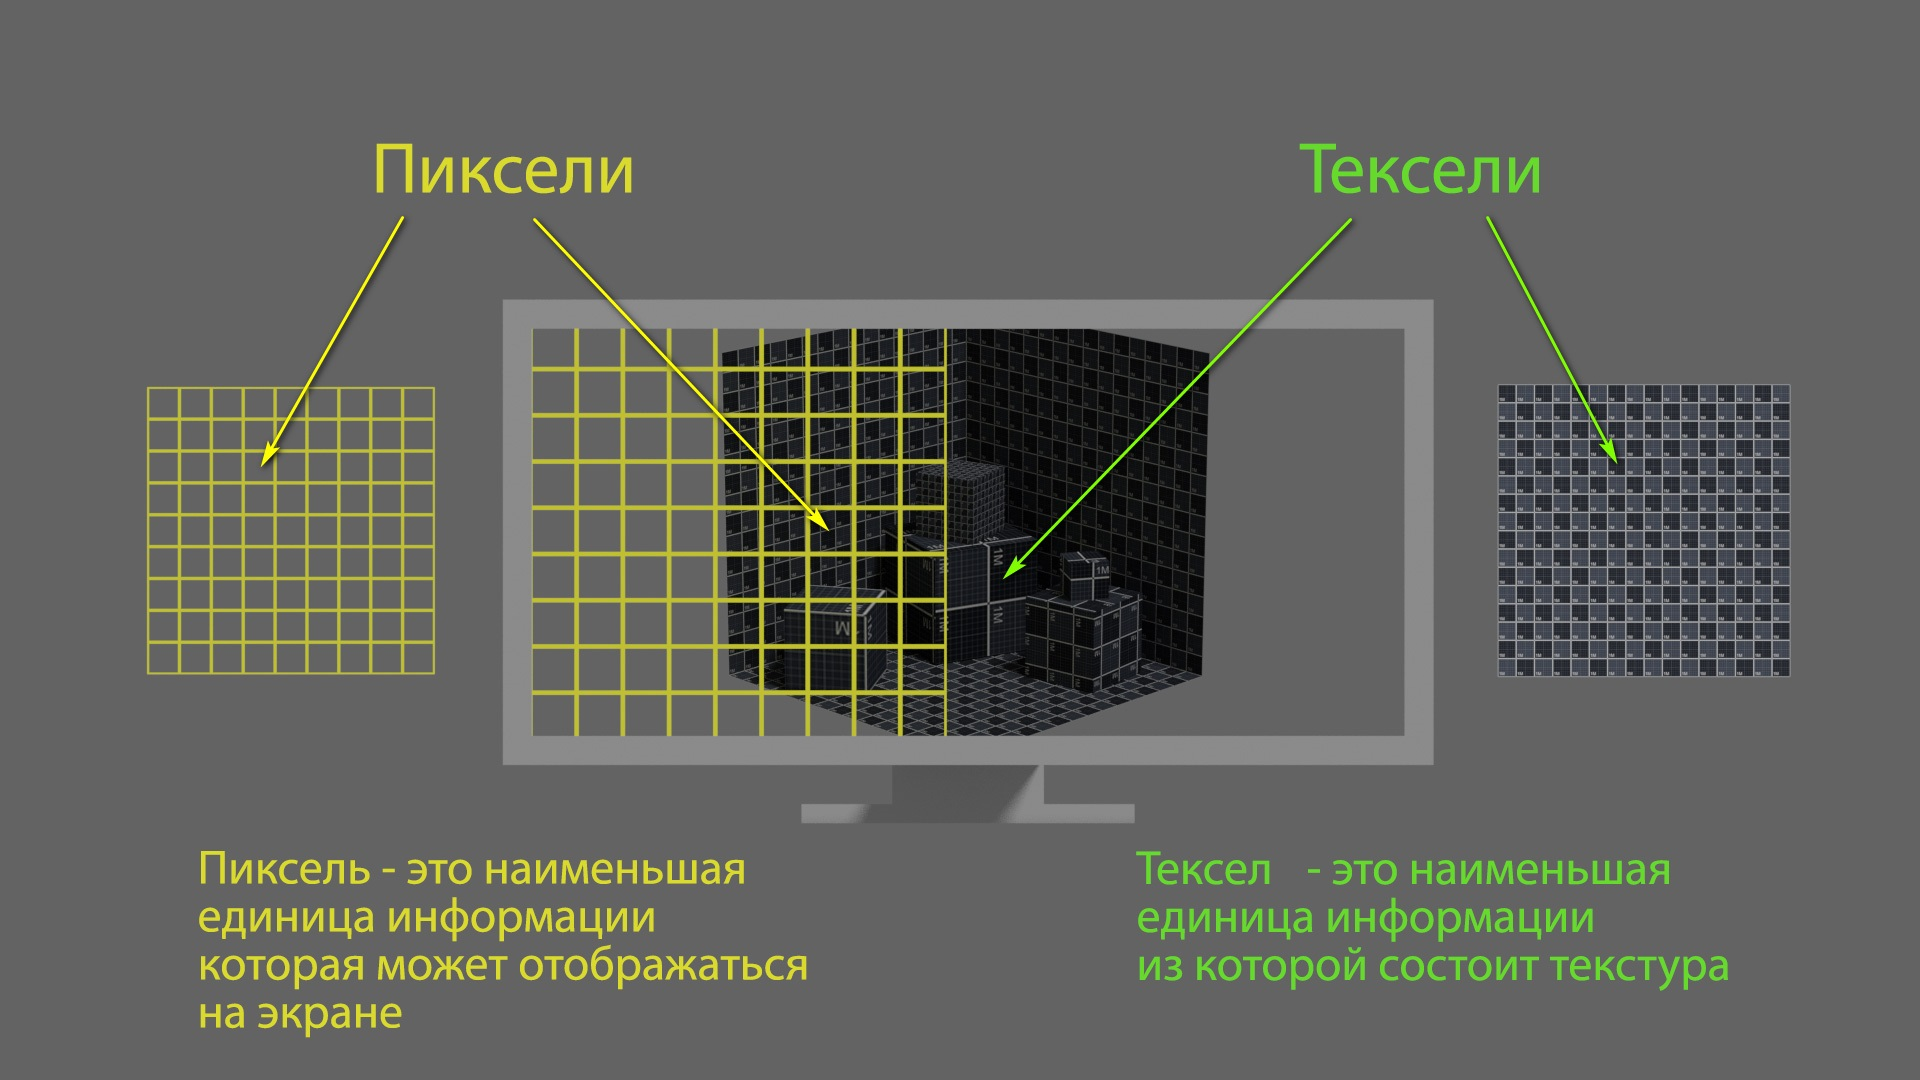
\includegraphics[width=0.9\textwidth]{images/texel.jpg}
				\caption{Пример текстуры}
			\end{figure}
		}
	\end{frame}

	\begin{frame}{Наложение текстур}{Texture Mapping}

		Пространство текстуры \\
		% texture space
		Координаты текстур \\
		uv-space

		{\hfill
			Преобразование поверхностной текстуры
		}

		Пространство объектов \\
		% object space
		Параметры поверхности \\
		xyz-space
		
		{\hfill
			Преобразование наблюдения, проецирования, растеризация
		}
		
		Пространство изображений \\
		% screen space
		Координаты пикселей \\
		xy-space
		
		\note{
			\begin{figure} 
				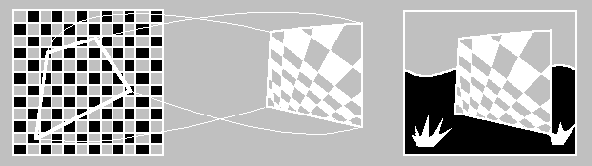
\includegraphics[width=\textwidth]{images/mapping.png}
				% 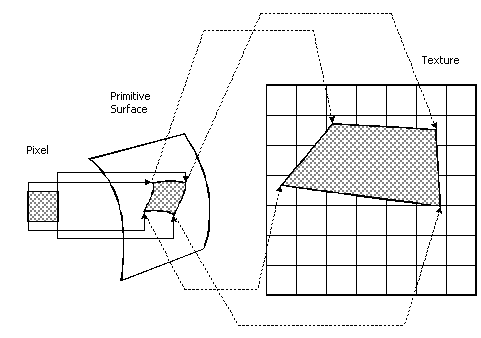
\includegraphics[width=0.4\textwidth]{images/texture_mapping.png}
				\caption{Пример текстуры}
			\end{figure}

			Примечание. \\
			направление наложения \\
			объект проецируется на текстуре

			Параметрическое преобразование
		}
		% https://learn.microsoft.com/en-us/windows/win32/direct3d9/texture-coordinates

	\end{frame}

	\begin{frame}{GPU Pipeline}

		Слайды с конвейером трехмерного преобразования
		L1-Introduction и L5-Graphics\_pipeline.
		% Vertex Shader \\
		% Rasterizer \\
		% Fragment Shader and Texture Unit \\
		% Image

		% \note{
		% 	\begin{figure} 
		% 		\includegraphics[width=0.9\textwidth]{images/}
		% 		\caption{Пример текстуры}
		% 	\end{figure}
		% }
	\end{frame}

	\begin{frame}{Эффект ступенчатости}{Aliasing}
		Термин "aliasing" (ступенчатость) происходит от слова "alias"\ в английском языке, которое означает "псевдоним"\ или "иное имя". 
		
		{\footnotesize
		В компьютерной графике, алиасинг происходит, когда высокочастотные детали изображения (например, тонкие линии или края) не могут быть правильно представлены на низкочастотной сетке пикселей. 
		Это приводит к появлению артефактов в виде ступенчатости или "псевдонимов"\ вдоль краев объектов. 
		%Антиалиасинг, как техника, направленная на уменьшение этих ступенчатых эффектов, призвана устранять или смягчать эти "псевдонимы" на изображениях, делая их более гладкими и природными визуально.
		}
		
		Антиалиасинг (англ. antialiasing) - это техника в компьютерной графике, направленная на уменьшение ступенчатости (или зубчатости) на изображениях, особенно заметной на краях объектов или диагоналях. 
				
		{\footnotesize
		Ступенчатость возникает из-за ограниченного числа пикселей, используемых для представления изображения, что может создавать впечатление неровных и недостаточно гладких линий.
		Антиалиасинг достигается путем размытия переходов между цветами на краях объектов. Это может быть выполнено различными методами, включая сглаживание, суперсэмплирование и другие. %Результатом является более гладкое и естественное визуальное восприятие изображения.
		}
		\note{
			% https://www.pcmag.com/encyclopedia/term/anti-aliasing
			\begin{figure} 
				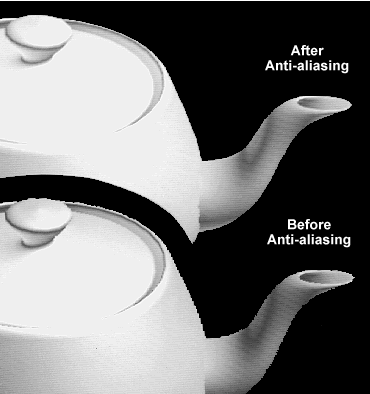
\includegraphics[width=0.5\textwidth]{images/anti-aliasing.png}
				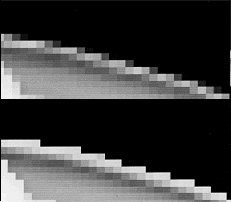
\includegraphics[width=0.45\textwidth]{images/anti-aliasing_extra.png}
				\caption{Пример текстуры}
			\end{figure}
		}

	\end{frame}

	\begin{frame}{Текстуры}

		Способы наложения текстуры 
		\begin{enumerate}
			\item метод ближайшей точки (без фильтрации)
			\item билинейная фильтрация 
			\item бикубическая фильтрация
			\item трилинейная фильтрация 
			\item анизотропная фильтрация 
		\end{enumerate}

		\note{
			% https://kwojcicki.github.io/blog/NEAREST-NEIGHBOUR
			\begin{figure} 
				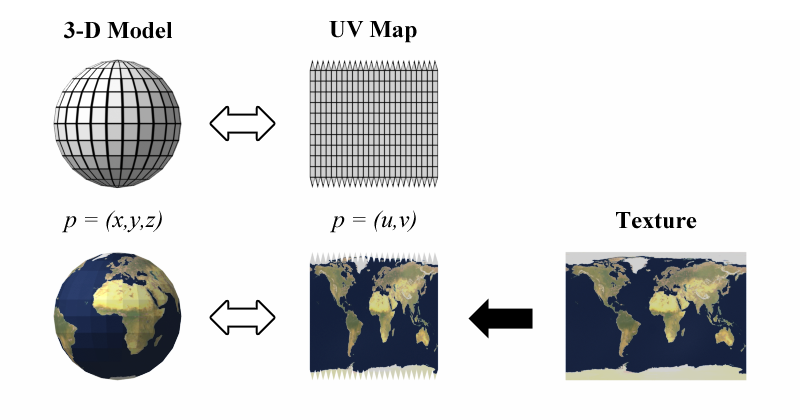
\includegraphics[width=0.8\textwidth]{images/UVMapping.png}
				\caption{uv-развертка (uv-mapping) }
			\end{figure}
		}
	\end{frame}

	\begin{frame}{Метод ближайшего соседа}{Nearest-Neighbour Method}

	 	Метод ближайшего соседа --- основан на ступенчатой интерполяции.

		Этот метод использует значения самого близкого пикселя для вычисления нового значения после масштабирования.

		Когда изображение масштабируется в больший размер, каждый новый пиксель получает значение из ближайшего пикселя в оригинальном изображении. Аналогично, при уменьшении размера каждый новый пиксель получает значение из ближайшего пикселя, что может быть менее точным представлением данных.
				
		Вот примеры использования метода ближайшего соседа:
		
		\begin{enumerate}
			\item 
			Приложения с низкими требованиями к производительности;
			\item 
			Бинарные изображения (черно-белые; только два цвета).
		\end{enumerate}




		% методом ближайшего соседа (ступенчатая интерполяция) —
		% $P_1; P_2; P_3$
		% качество
		% Nearest Texel for current Pixel
		% example
		% $u = \alpha u_0 + \beta u_1 + \gamma u_2$
		\note{
			% https://kwojcicki.github.io/blog/NEAREST-NEIGHBOUR
			\begin{figure} 
				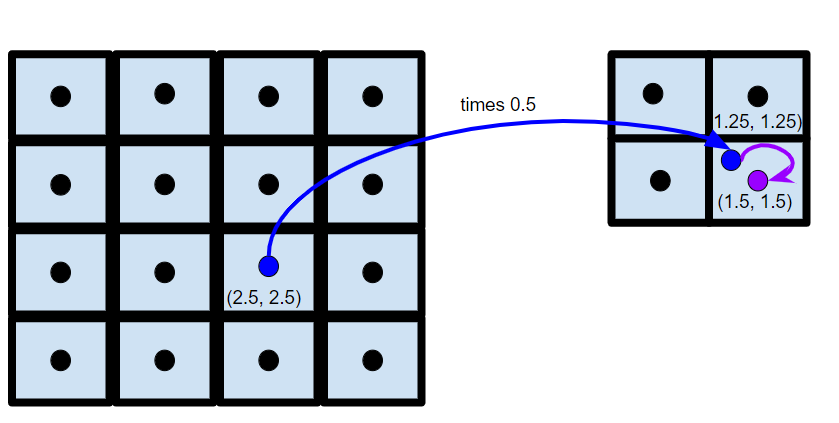
\includegraphics[width=0.8\textwidth]{images/nn_filtering.png}
				\caption{Пример текстуры}
			\end{figure}
		}

		% https://community.adobe.com/t5/substance-3d-painter-discussions/viewport-texturing-filtering/td-p/13444697
		
	\end{frame}
	
	\begin{frame}{Текстурная фильтрация}{Texture Filtering}
		Фильтрации основаны на интерполяции
		% Interpolation
		
		% Bilinear Filtering
		Билинейная фильтрация --- это метод фильтрации текстур в компьютерной графике, используемый для улучшения качества отображения текстур при масштабировании. Этот метод предназначен для устранения ступенчатости и артефактов, которые могут возникнуть при изменении размера текстур.


		% Bicubic Filtering
		Бикубическая фильтрация --- это метод фильтрации, используемый в компьютерной графике, который обеспечивает более точное и качественное увеличение изображений и текстур по сравнению с билинейной фильтрацией. Этот метод часто применяется при изменении размера изображений.

		{\footnotesize
			Основная идея бикубической фильтрации заключается в том, чтобы использовать значения не только ближайших пикселей, как в билинейной фильтрации, но и значения соседних пикселей, чтобы создать более гладкие и точные результаты. Алгоритм использует кубические полиномы для интерполяции значений пикселей.
		}

		% Слайды с конвейером трехмерного преобразования
		% L1-Introduction и L5-Graphics\_pipeline.

		\note{
			\begin{figure} 
				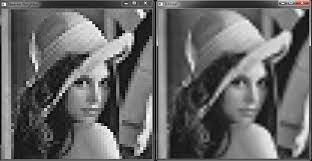
\includegraphics[width=\textwidth]{images/bilinear_filtering.jpg}
				\caption{Сравнение фильтрации методом ближайшего соседа и билинейной фильтрации}
			\end{figure}
		}

	\end{frame}

	\begin{frame}{Mip-текстура}{Mipmaps}
		
		Mipmap (Multum In Parvo, Многое в малом) представляет собой предварительно созданный набор изображений с разными разрешениями исходной текстуры. Каждое последующее изображение в этом наборе имеет размер в половину (или в другой пропорции) меньший, чем предыдущее. Таким образом, создается иерархия текстур, где каждый уровень представляет собой изображение с определенным уровнем детализации.

		Использование такой текстуры позволяет избежать артефактов, таких как мерцание и дрожание текстур на дальних объектах, и в то же время повысить производительность при рендеринге.
		% 		MIP-mapping увеличивает расход видеопамяти на треть:
		% 	\[
		% 		\sum_{i=0}^\infty \left( \frac {1} {4} \right)^i = 1 \frac {1} {3}
		% 	\]

		% При наложении текстур вычисляется расстояние до объекта и номер текстуры находится по формуле:
		% \[
		% 	{mip\_level} = \log_2 \left( \frac {{distance}} {{texel\_size} \cdot {camera\_resolution}} \right) + {mip\_bias}
		% 	,
		% 	\]
		% 	$mip\_bias$ --- число, позволяющее выбирать более или менее детальную текстуру, чем даёт формула.
		% где $resolution$ --- разрешение виртуальной камеры (количество пикселей, которое будет в объекте размером в 1 ед., расположенном в 1 ед. от камеры), $texelsize$ --- размер текселя в единицах трёхмерного мира, $dist$ --- расстояние до объекта в тех же единицах, 
		% Это число округляется до целого, и текстура с соответствующим номером (нулевая — самая детальная, первая — вдвое меньшая и т. д.) накладывается на объект.

		\note{
			\begin{figure} 
				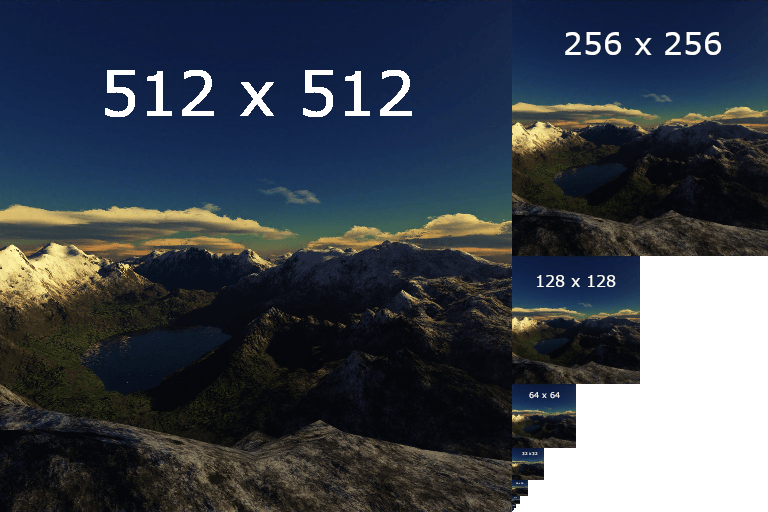
\includegraphics[width=0.75\textwidth]{images/mipmap.png}
				\caption{Mip-текстура}
			\end{figure}
		}

	\end{frame}

	\begin{frame}{Трилинейная фильтрация}{Trilinear Filter}
		Трилинейная фильтрация --- это техника фильтрации текстур в компьютерной графике, предназначенная для улучшения качества отображения при масштабировании текстур на различных расстояниях и углах обзора.

		Трилинейная фильтрация включает в себя два этапа фильтрации:
		\begin{enumerate}
			\item 
			Мипмап фильтрация: Выбор подходящего уровня mipmap в зависимости от расстояния до объекта.
			\item
			Билинейная фильтрация: Интерполяция значений внутри выбранного уровня mipmap.
		\end{enumerate}


		Трилинейная фильтрация обеспечивает более гладкое и качественное отображение текстур, особенно при масштабировании, так как она учитывает как изменения масштаба, так и углы обзора.

		Недостаток такой техники заключается в том, что все цвета вдалеке сильно смешиваются.

		\note{
			\begin{figure} 
				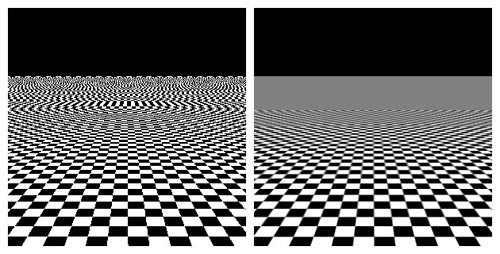
\includegraphics[width=\textwidth]{images/bi_tri_linear_filtering.jpg}
				\caption{Сравнение билинейной и трилинейной фильтраций}
			\end{figure}
		}

	\end{frame}


	
	
	\begin{frame}{Анизатропная фильтрация}{Anisotropic Filtering (with Mipmaps)}


		
		Анизотропная фильтрация --- это техника в компьютерной графике, применяемая к текстурам для улучшения качества отображения при различных углах обзора. Эта техника особенно полезна при работе с текстурами, которые наклонены под разными углами или отображаются под разными ракурсами.
		
		Фактически убирает размытие при смешивании за счет того, что работает в трех измерениях.
		
		% Преимущества анизотропной фильтрации включают:
		
		% 		Качество отображения: Улучшение качества текстур при различных углах обзора, что особенно важно для текстур, ориентированных под углом к камере.
		
		% 		Плавные переходы: Снижение артефактов, таких как ступенчатость, и обеспечение более плавных переходов между пикселями текстуры.
		
		% 		Более точное отображение деталей: Анизотропная фильтрация позволяет более точно отобразить детали текстур, особенно при масштабировании.
		
		% Однако использование анизотропной фильтрации может быть более ресурсоемким процессом по сравнению с обычной билинейной фильтрацией, поэтому ее применяют там, где требуется более высокое качество отображения.
	
		\note{
			\begin{figure} 
				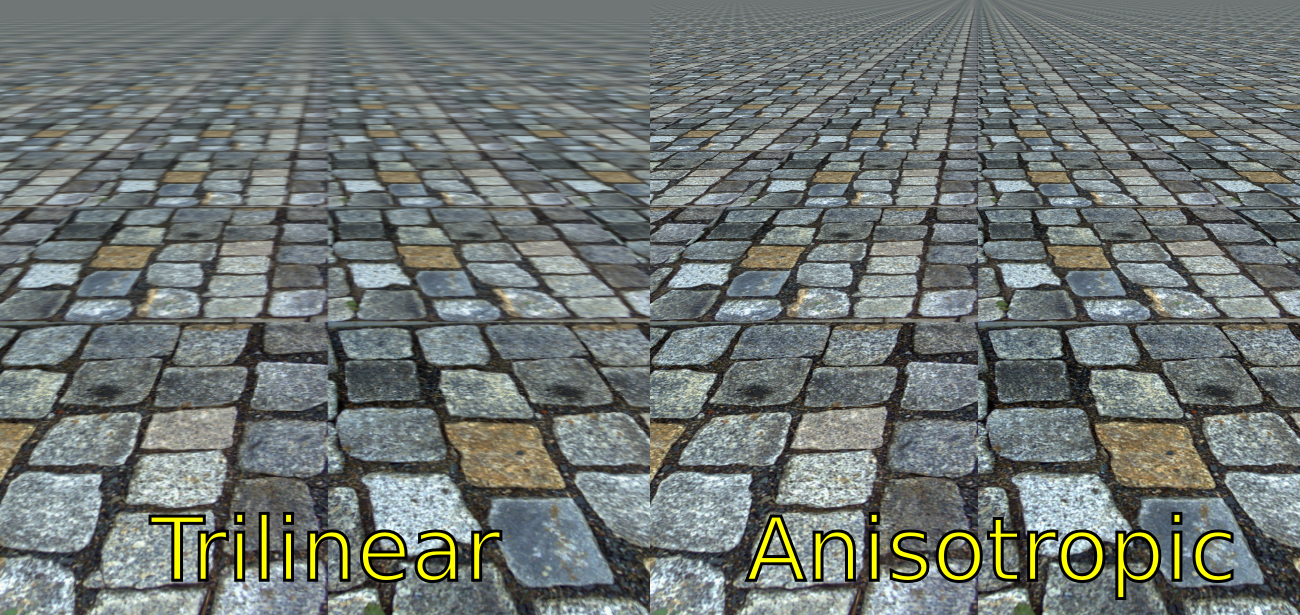
\includegraphics[width=\textwidth]{images/anisotropic_filtering.png}
				\caption{Сравнение трилинейной и анизатропной фильтраций}
			\end{figure}
		}


	\end{frame}


	\begin{frame}{Классификация}

		Основные виды
		\begin{enumerate}
			\item Исходные изображения;
			\item MIP-текстуры;
			\item Процедурные текстуры. %Procedural Textures c=f(u) флаги
			%working set попадают в текстурную память
		\end{enumerate}
		
		Специализированные
		\begin{enumerate}
			\item Карта нормалей (Normal Map);
			\item Карта высот (Height Map);
			
			\item Карта окклюзии (Ambient Occlusion Map);
			\item Карта тени (Shadow Map);
		
			\item Карта смешивания (Blend Map);
		\end{enumerate}

		\note{
			Эффект наложения текстур на полигональные модели привел к большому прорыву. 
			\\До сих пор использование текстур является основой для построения реалистичного изображения. %Количество видов поражает!
		}
	\end{frame}

	\begin{frame}{Процедурные текстуры}

		Процедурные текстуры - это текстуры, которые генерируются алгоритмически, а не создаются вручную или с помощью изображений. 
		Они используют математические функции и алгоритмы для создания деталей, шумов, узоров и других характеристик текстуры. Этот подход позволяет создавать бесконечные и вариативные текстуры, которые могут быть адаптированы под различные условия и среды.

Примеры процедурных текстур:
\begin{enumerate}
	\item 
	Шум Перлина (Perlin Noise)%: Это один из наиболее распространенных алгоритмов для генерации текстурного шума, используемого в компьютерной графике и компьютерной генерации изображений. Он может быть использован для создания реалистичных поверхностей, таких как горы, облака, вода и др.
	\item
	Фрактальные текстуры%: Алгоритмы фрактальной генерации могут быть использованы для создания текстур с самоподобными деталями на различных уровнях масштаба. Это может быть полезно для создания разнообразных природных элементов, таких как леса, горы и т. д.
	\item
	Текстуры шероховатости%: Процедурные алгоритмы могут быть использованы для создания текстур с различными уровнями шероховатости, что может быть полезно для реализации реалистичных материалов, таких как камень, дерево и т. д.
	\item
	Марблинг и деревообразные текстуры%: Процедурные текстуры могут эмулировать множество различных природных и искусственных материалов, таких как мрамор, дерево, металл и другие.
\end{enumerate}

	Преимущество процедурных текстур заключается в их гибкости, возможности легкой настройки и создания уникальных вариантов текстур без необходимости хранения больших файлов изображений.

		\note{
			% http://www.upvector.com/?section=Tutorials&subsection=Intro%20to%20Procedural%20Textures
				\begin{figure} 
					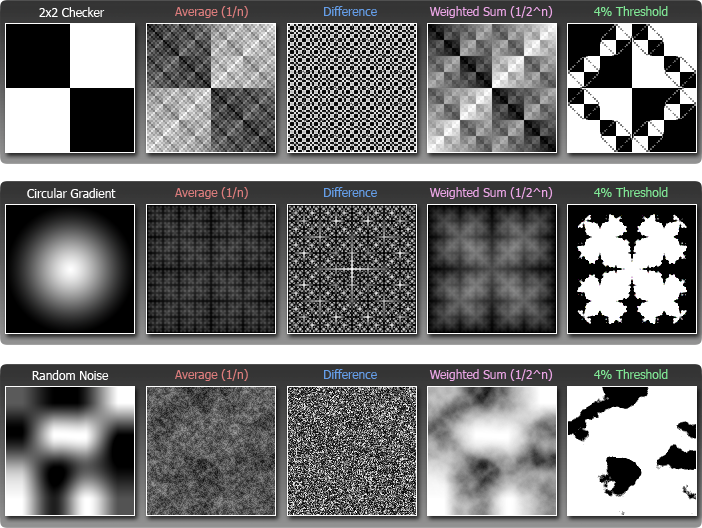
\includegraphics[width=0.7\textwidth]{images/procedural_textures.png}
					\caption{Процедурные текстуры}
				\end{figure}
		}
	\end{frame}


	\begin{frame}{Специализированные текстуры}
		\begin{enumerate}
			\item Карта нормалей (Normal Map): Используется для добавления деталей к поверхности объекта, не увеличивая количество полигонов. Цвет каждого пикселя карты нормалей представляет собой вектор, указывающий направление нормали к поверхности в данной точке.
			% https://ycpcs.github.io/cs470-fall2014/labs/lab12-2.html
			\item Карта высот (Height Map): Используется для создания рельефности поверхности. Значения яркости пикселей определяют высоту соответствующих точек на поверхности объекта.
			%\item Карта выпуклостей (Bump map): используется для создания иллюзии высоких и низких точек на поверхности, но без фактического изменения геометрии. Он воздействует на освещение, создавая тени и подчеркивая детали, но не изменяет форму самого объекта.
	
		\end{enumerate}


		
		\note{
			% https://typhen.artstation.com/blog/BDr6/this-is-normal-2-baking-normal-maps
			\begin{figure} 
				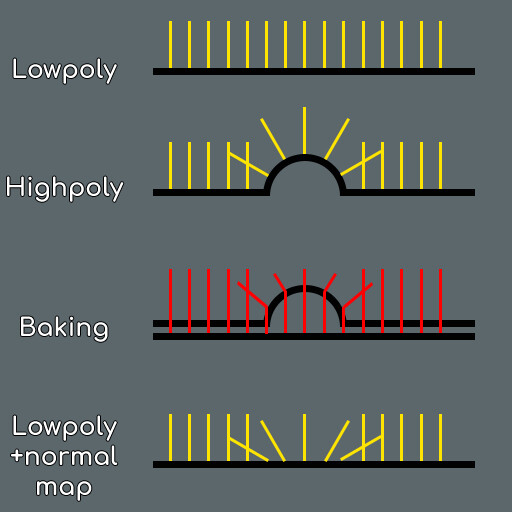
\includegraphics[width=0.45\textwidth]{images/Baking.jpg}
				\caption{Запекание текстуры}
			\end{figure}
		}
	\end{frame}

	\begin{frame}{Специализированные текстуры}{связанные с тенями}
		\begin{enumerate}
			\item Карта окклюзии (Ambient Occlusion Map): Описывает, насколько освещен каждый пиксель, учитывая его окружение. Темные области могут указывать на близость объектов или узкие пространства, где освещение ограничено.
			\item Карта тени (Shadow Map): Используется для определения областей, находящихся в тени. 
		\end{enumerate}
		
		Примечание.
		\\Текстура, в которой хранятся тени от рассеянного света, содержит оттенки серого.
		\\ Подходит для сцены с неподвижными источниками света.
	
			\note{
				% https://3dclub.com/blog/kak-ispolzovat-karty-ao
				% https://gamedev.ru/code/forum/?id=175200
				\begin{figure} 
					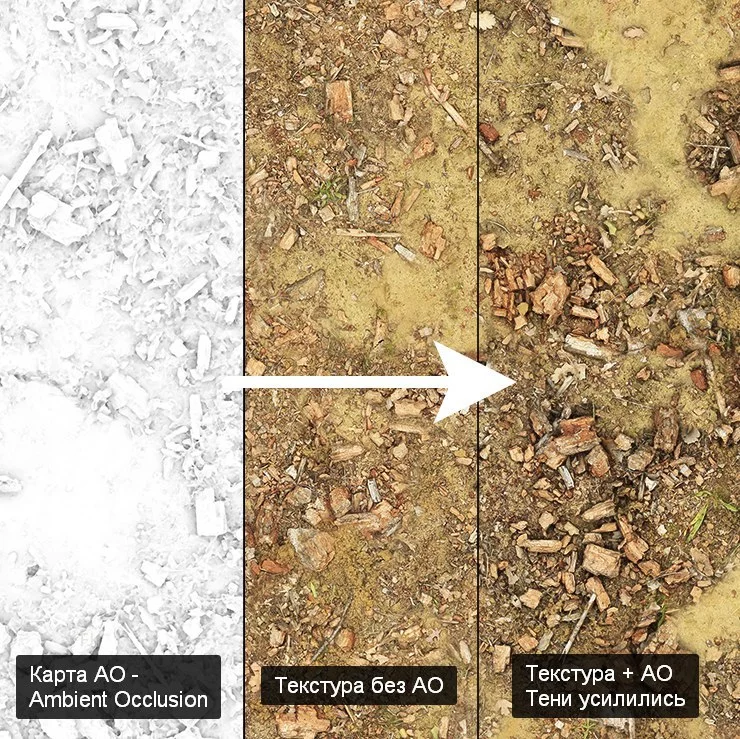
\includegraphics[width=0.45\textwidth]{images/ambient_occlusion.png}
					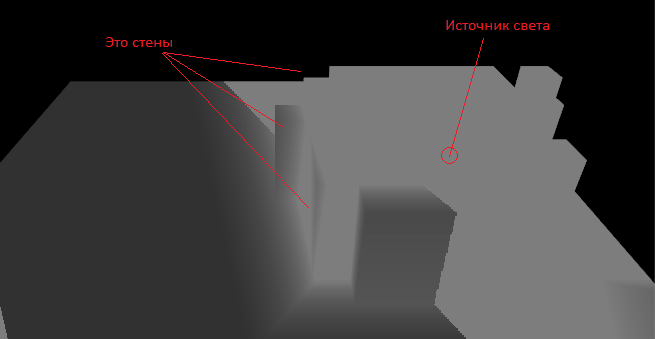
\includegraphics[width=0.5\textwidth]{images/shadow_mapping.png}
					\caption{Ambient Occlusion Map и карта теней}
				\end{figure}
			}
	\end{frame}

	\begin{frame}{Специализированные текстуры}
		\begin{enumerate}		
			\item Карта смешивания (Blend Map): Применяется для смешивания нескольких текстур в зависимости от определенных условий. Например, можно использовать карту смешивания для определения, где на объекте применять текстуру травы, а где текстуру камня.
			\end{enumerate}

			\begin{figure} 
				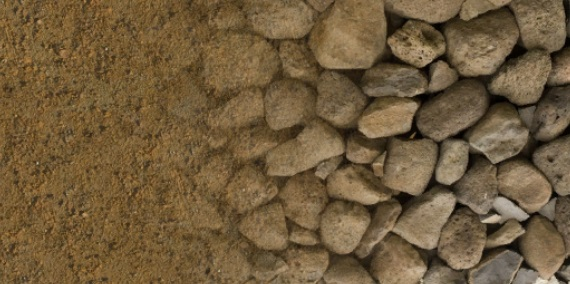
\includegraphics[width=0.5\textwidth]{images/blend_1.jpg}
				\caption{Проблема при смешивании}
			\end{figure}

			% https://habr.com/ru/articles/180743/
			\note{
				\begin{figure}
					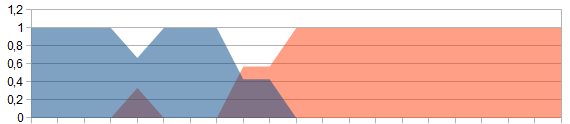
\includegraphics[width=0.7\textwidth]{images/blend_4.png}
					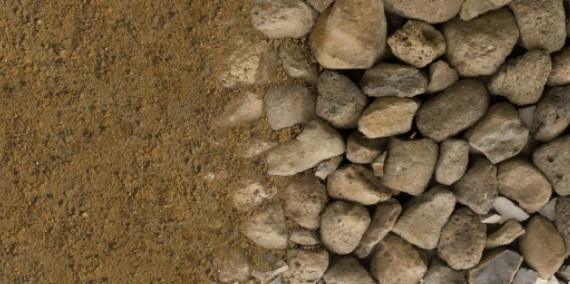
\includegraphics[width=0.7\textwidth]{images/blend_3.jpg}
					\caption{Карта смешивания и результат}
				\end{figure}
	
			}

	\end{frame}

	\begin{frame}{Заключение}
		Литература
		\begin{enumerate}
			\item \href{http://www.upvector.com/?section=Tutorials&subsection=Intro\ to\ Procedural\ Textures}{Procedural Textures}
			\item \href{http://euklid.mi.uni-koeln.de/c/mirror/www.cs.curtin.edu.au/units/cg351-551/notes/lect9i1.html}{Displaying Textures on the Screen}
			\item \href{https://learn.microsoft.com/en-us/windows/win32/direct3d9/texture-coordinates}{Texture Coordinates}
			\item \href{https://www.pcmag.com/encyclopedia/term/anti-aliasing}{Anti-Aliasing}
			\item \href{https://kwojcicki.github.io/blog/NEAREST-NEIGHBOUR}{Nearest Neighbour Interpolation}
			\item \href{https://community.adobe.com/t5/substance-3d-painter-discussions/viewport-texturing-filtering/td-p/13444697}{Viewport Texturing Filtering}
			% \item \href{http://www.upvector.com/?section=Tutorials&subsection=Intro to Procedural\ Textures}{text}
			\item \href{https://ycpcs.github.io/cs470-fall2014/labs/lab12-2.html}{Normal and Displacement Mapping}
			\item \href{https://typhen.artstation.com/blog/BDr6/this-is-normal-2-baking-normal-maps}{Baking Normal Maps}
			\item \href{https://3dclub.com/blog/kak-ispolzovat-karty-ao}{Что такое Ambient Occlusion}
			\item \href{https://gamedev.ru/code/forum/?id=175200}{Shadow Mapping}
			\item \href{https://habr.com/ru/articles/180743}{Смешивание текстур ландшафта}
		\end{enumerate}

	\end{frame}

	\end{document}